%%%%%%%%%%%%%%%%%%%%%%%%%%%%%%%%%%%%%%%%%
% Beamer Presentation
% LaTeX Template
% Version 1.0 (10/11/12)
%
% This template has been downloaded from:
% http://www.LaTeXTemplates.com
%
% License:
% CC BY-NC-SA 3.0 (http://creativecommons.org/licenses/by-nc-sa/3.0/)
%
%%%%%%%%%%%%%%%%%%%%%%%%%%%%%%%%%%%%%%%%%

%----------------------------------------------------------------------------------------
%	PACKAGES AND THEMES
%----------------------------------------------------------------------------------------

\documentclass{beamer}

\mode<presentation> {

% The Beamer class comes with a number of default slide themes
% which change the colors and layouts of slides. Below this is a list
% of all the themes, uncomment each in turn to see what they look like.

%\usetheme{default}
%\usetheme{AnnArbor}
%\usetheme{Antibes}
%\usetheme{Bergen}
%\usetheme{Berkeley}
%\usetheme{Berlin}
%\usetheme{Boadilla}
%\usetheme{CambridgeUS}
%\usetheme{Copenhagen}
%\usetheme{Darmstadt}
%\usetheme{Dresden}
%\usetheme{Frankfurt}
%\usetheme{Goettingen}
%\usetheme{Hannover}
%\usetheme{Ilmenau}
%\usetheme{JuanLesPins}
%\usetheme{Luebeck}
\usetheme{Madrid}
%\usetheme{Malmoe}
%\usetheme{Marburg}
%\usetheme{Montpellier}
%\usetheme{PaloAlto}
%\usetheme{Pittsburgh}
%\usetheme{Rochester}
%\usetheme{Singapore}
%\usetheme{Szeged}
%\usetheme{Warsaw}

% As well as themes, the Beamer class has a number of color themes
% for any slide theme. Uncomment each of these in turn to see how it
% changes the colors of your current slide theme.

%\usecolortheme{albatross}
%\usecolortheme{beaver}
%\usecolortheme{beetle}
%\usecolortheme{crane}
%\usecolortheme{dolphin}
%\usecolortheme{dove}
%\usecolortheme{fly}
%\usecolortheme{lily}
%\usecolortheme{orchid}
%\usecolortheme{rose}
%\usecolortheme{seagull}
%\usecolortheme{seahorse}
%\usecolortheme{whale}
%\usecolortheme{wolverine}

%\setbeamertemplate{footline} % To remove the footer line in all slides uncomment this line
%\setbeamertemplate{footline}[page number] % To replace the footer line in all slides with a simple slide count uncomment this line

%\setbeamertemplate{navigation symbols}{} % To remove the navigation symbols from the bottom of all slides uncomment this line
}

\usepackage{graphicx} % Allows including images
\usepackage{booktabs} % Allows the use of \toprule, \midrule and \bottomrule in tables

% \usepackage{animate,media9,movie15}
\renewcommand{\footnotesize}{\fontsize{6pt}{11pt}}


%----------------------------------------------------------------------------------------
%	TITLE PAGE
%----------------------------------------------------------------------------------------

\title[Brain dataset]{Final Report: Brain Dataset} % The short title appears at the bottom of every slide, the full title is only on the title page

\author{Roman Podolski, Philipp Bergmann, Dominik Irimi, Manuel Nickel, Christoph Dehner} % Your name
\institute[TUM] % Your institution as it will appear on the bottom of every slide, may be shorthand to save space
{
Technische Universit\"at M\"unchen \\ % Your institution for the title page
\medskip
\textit{roman.podolski@tum.de, philipp.bergmann@tum.de, dominik.irimi@tum.de, manuel.nickel@tum.de, dehner@in.tum.de} % Your email address
}
\date{\today} % Date, can be changed to a custom date

\begin{document}

\begin{frame}
\titlepage % Print the title page as the first slide
\end{frame}

\begin{frame}
\frametitle{Overview} % Table of contents slide, comment this block out to remove it
\tableofcontents % Throughout your presentation, if you choose to use \section{} and \subsection{} commands, these will automatically be printed on this slide as an overview of your presentation
\end{frame}

%----------------------------------------------------------------------------------------
%	PRESENTATION SLIDES
%----------------------------------------------------------------------------------------

%------------------------------------------------
\section{Dataset} % Sections can be created in order to organize your presentation into discrete blocks, all sections and subsections are automatically printed in the table of contents as an overview of the talk
%------------------------------------------------

%\subsection{Subsection Example} % A subsection can be created just before a set of slides with a common theme to further break down your presentation into chunks

\begin{frame}
        \frametitle{Dataset: WAY-EEG-GAL}
%WAY: Wearable interfaces for hAnd function recoverY\\
%GAL: Grasp And Lift\\
Experiment recording human grasp and lift tasks\footnote{Data source: \cite{eeg-emg-dataset}}

\begin{columns}
    \column{.65\textwidth}
	\begin{itemize}
        \item 3,936 grasp and lift trials
        \item 12 participants, 9 series recorded each
        \item EEG: 32 brain electrodes recorded at 5kHz
        \item EMG: 5 muscle sensors at 4kHz
        \item kinetic: 36 position/force signals at 500Hz
        \item grasp objects with different surface friction (silk/suede/sandpaper) or weight (165/330/660g)
    \end{itemize}
	\column{.35\textwidth}
    \begin{figure}[ht]
	    \centering
		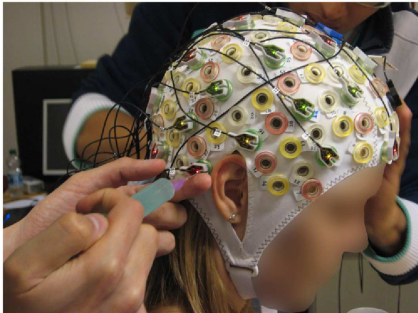
\includegraphics[width=1\textwidth, trim={3.5cm 1cm 1cm 1cm},clip]{images/eegelectrodes.png}
		\caption{EEG sensor cap}%\footnote{\cite{nature}}}
    \end{figure}
\end{columns}
\end{frame}


%\begin{frame}
%\frametitle{Experiment}
%
%Single trial procedure
%\begin{itemize}
%	\item start command signaled visually by LED
%	\item participant moves hand to object
%    \item grasp object
%    \item move object to target position
%    \item hold position
%    \item LED signal, to move object back to initial position
%    \item hand release object
%    \item move hand back to resting position
%\end{itemize}
%\end{frame}

\begin{frame}
    \frametitle{Experiment}
    \begin{figure}
%        \includemovie[autostart,continue,controls,poster,text={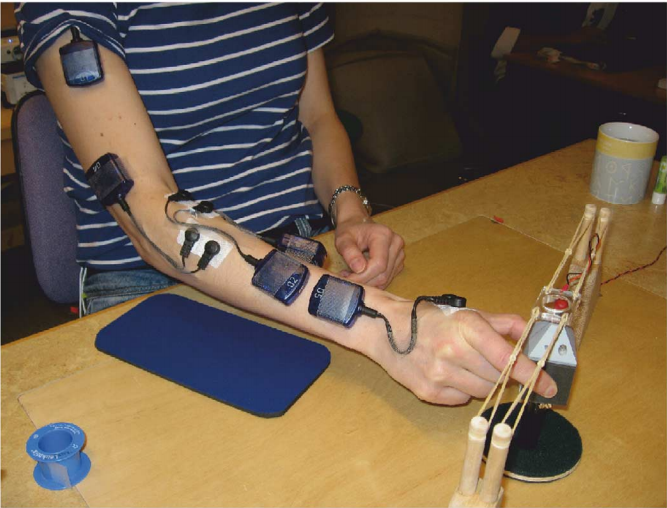
\includegraphics[scale=0.45]    {images/experiment.png}}]{6cm}{6cm}{images/sdata201447-s4.avi}
    \end{figure}
\end{frame}


\begin{frame}
	\frametitle{What this is all about}
	\textbf{What are we trying to do with this dataset?}\\
	\textbf{A:} We want to see if one can use EEG and EMG data to get an idea about the following issues: 
	
	\begin{itemize}
		\item Does a participant intend to grasp the object?
		\item Is he moving his hand \textbf{to} the object?
		\item Is he moving \textbf{back} to the resting position?
		\item Is he lifting the object?
		\item Is he holding an object?
	\end{itemize}
	
\end{frame}



%------------------------------------------------
\section{Analyzing the data}

\begin{frame}
	\frametitle{Analyzing the data using t-SNE}
	\textbf{Visualizing high-dimensional EMG and EEG data using t-SNE. Why?}
	\begin{itemize}
		\item Get a \emph{feeling} for the data
		\item See if notion of \emph{grasping} could possibly be captured by a Feedforward Neural Net
	\end{itemize}
	\begin{columns}
		\column{.7\textwidth}
		\begin{block}{Idea}
			\begin{itemize}
				\item \emph{Grasping}-states and \emph{Not Grasping}-states clustered respectively $\rightarrow$ Use Feedforward NN to classify \emph{Grasping}.
				\item No apparent structure in the plot $\rightarrow$ Use Recurrent NN.
			\end{itemize}
		\end{block}
		\column{.3\textwidth}
		\begin{figure}[ht]
			\centering
			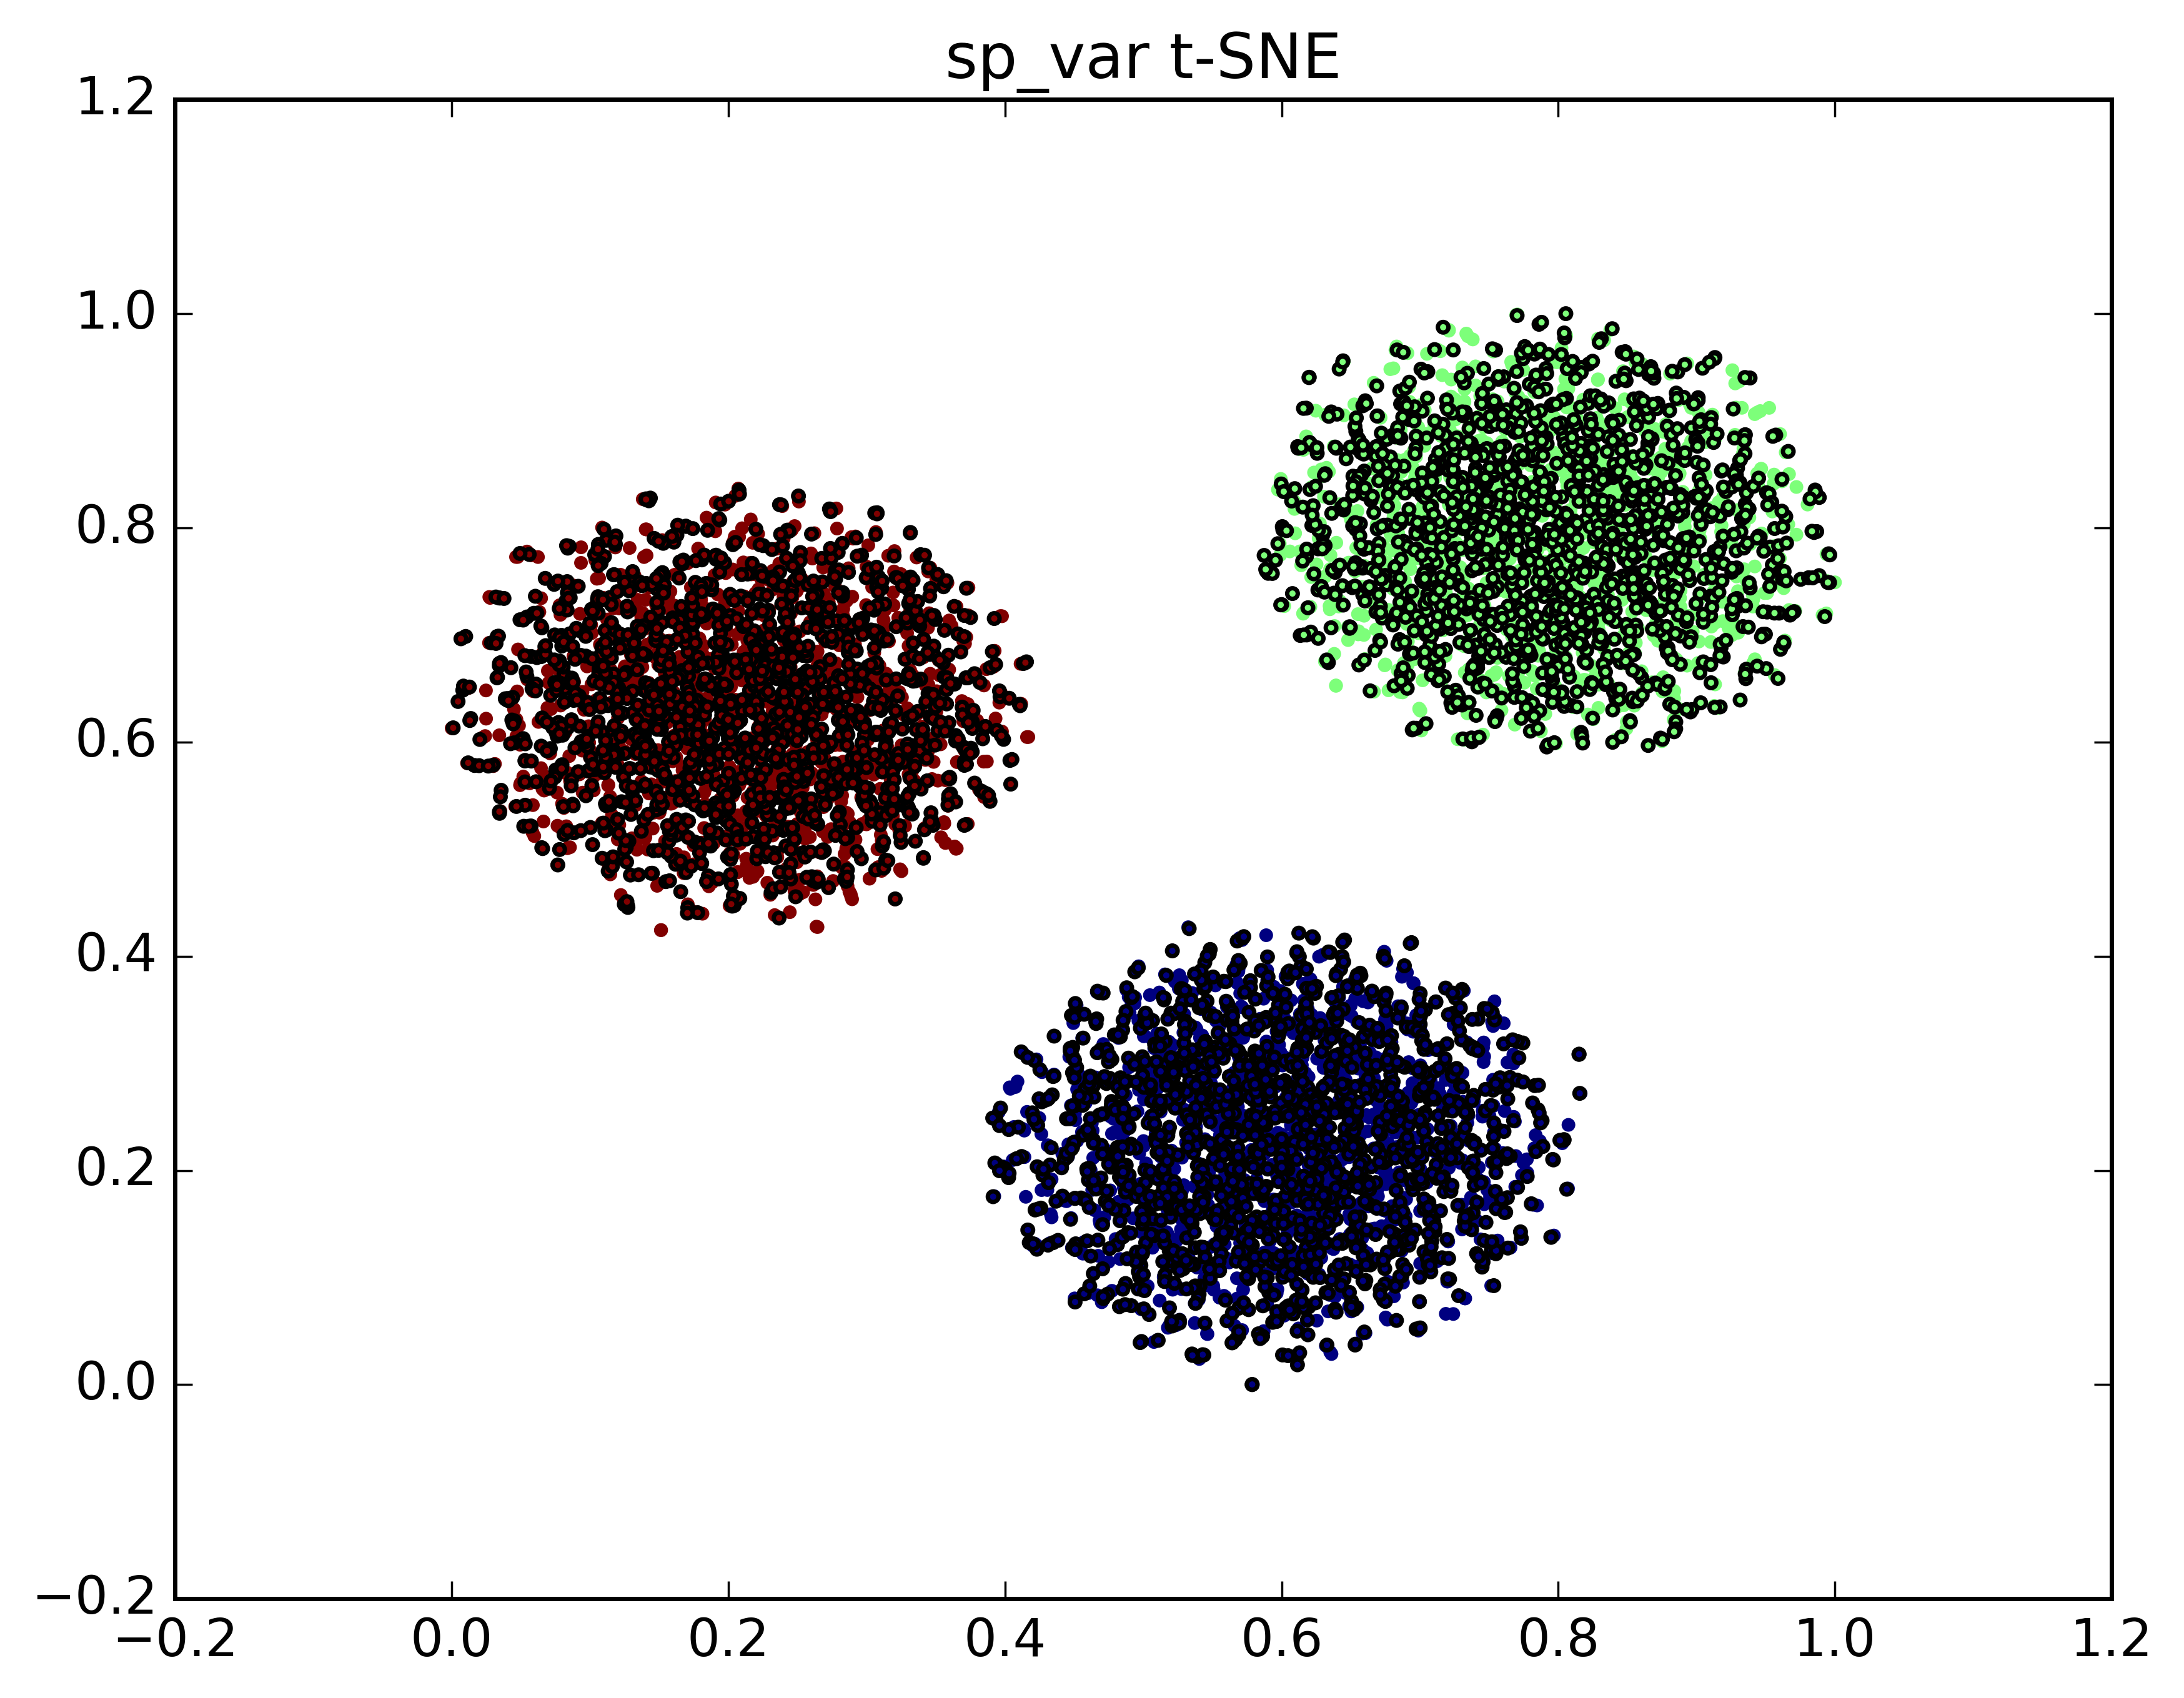
\includegraphics[width=0.8\textwidth, trim={2cm 2.5cm 2cm 2cm},clip]{images/cluster.png}
		\end{figure}
		\begin{figure}[ht]
			\centering
			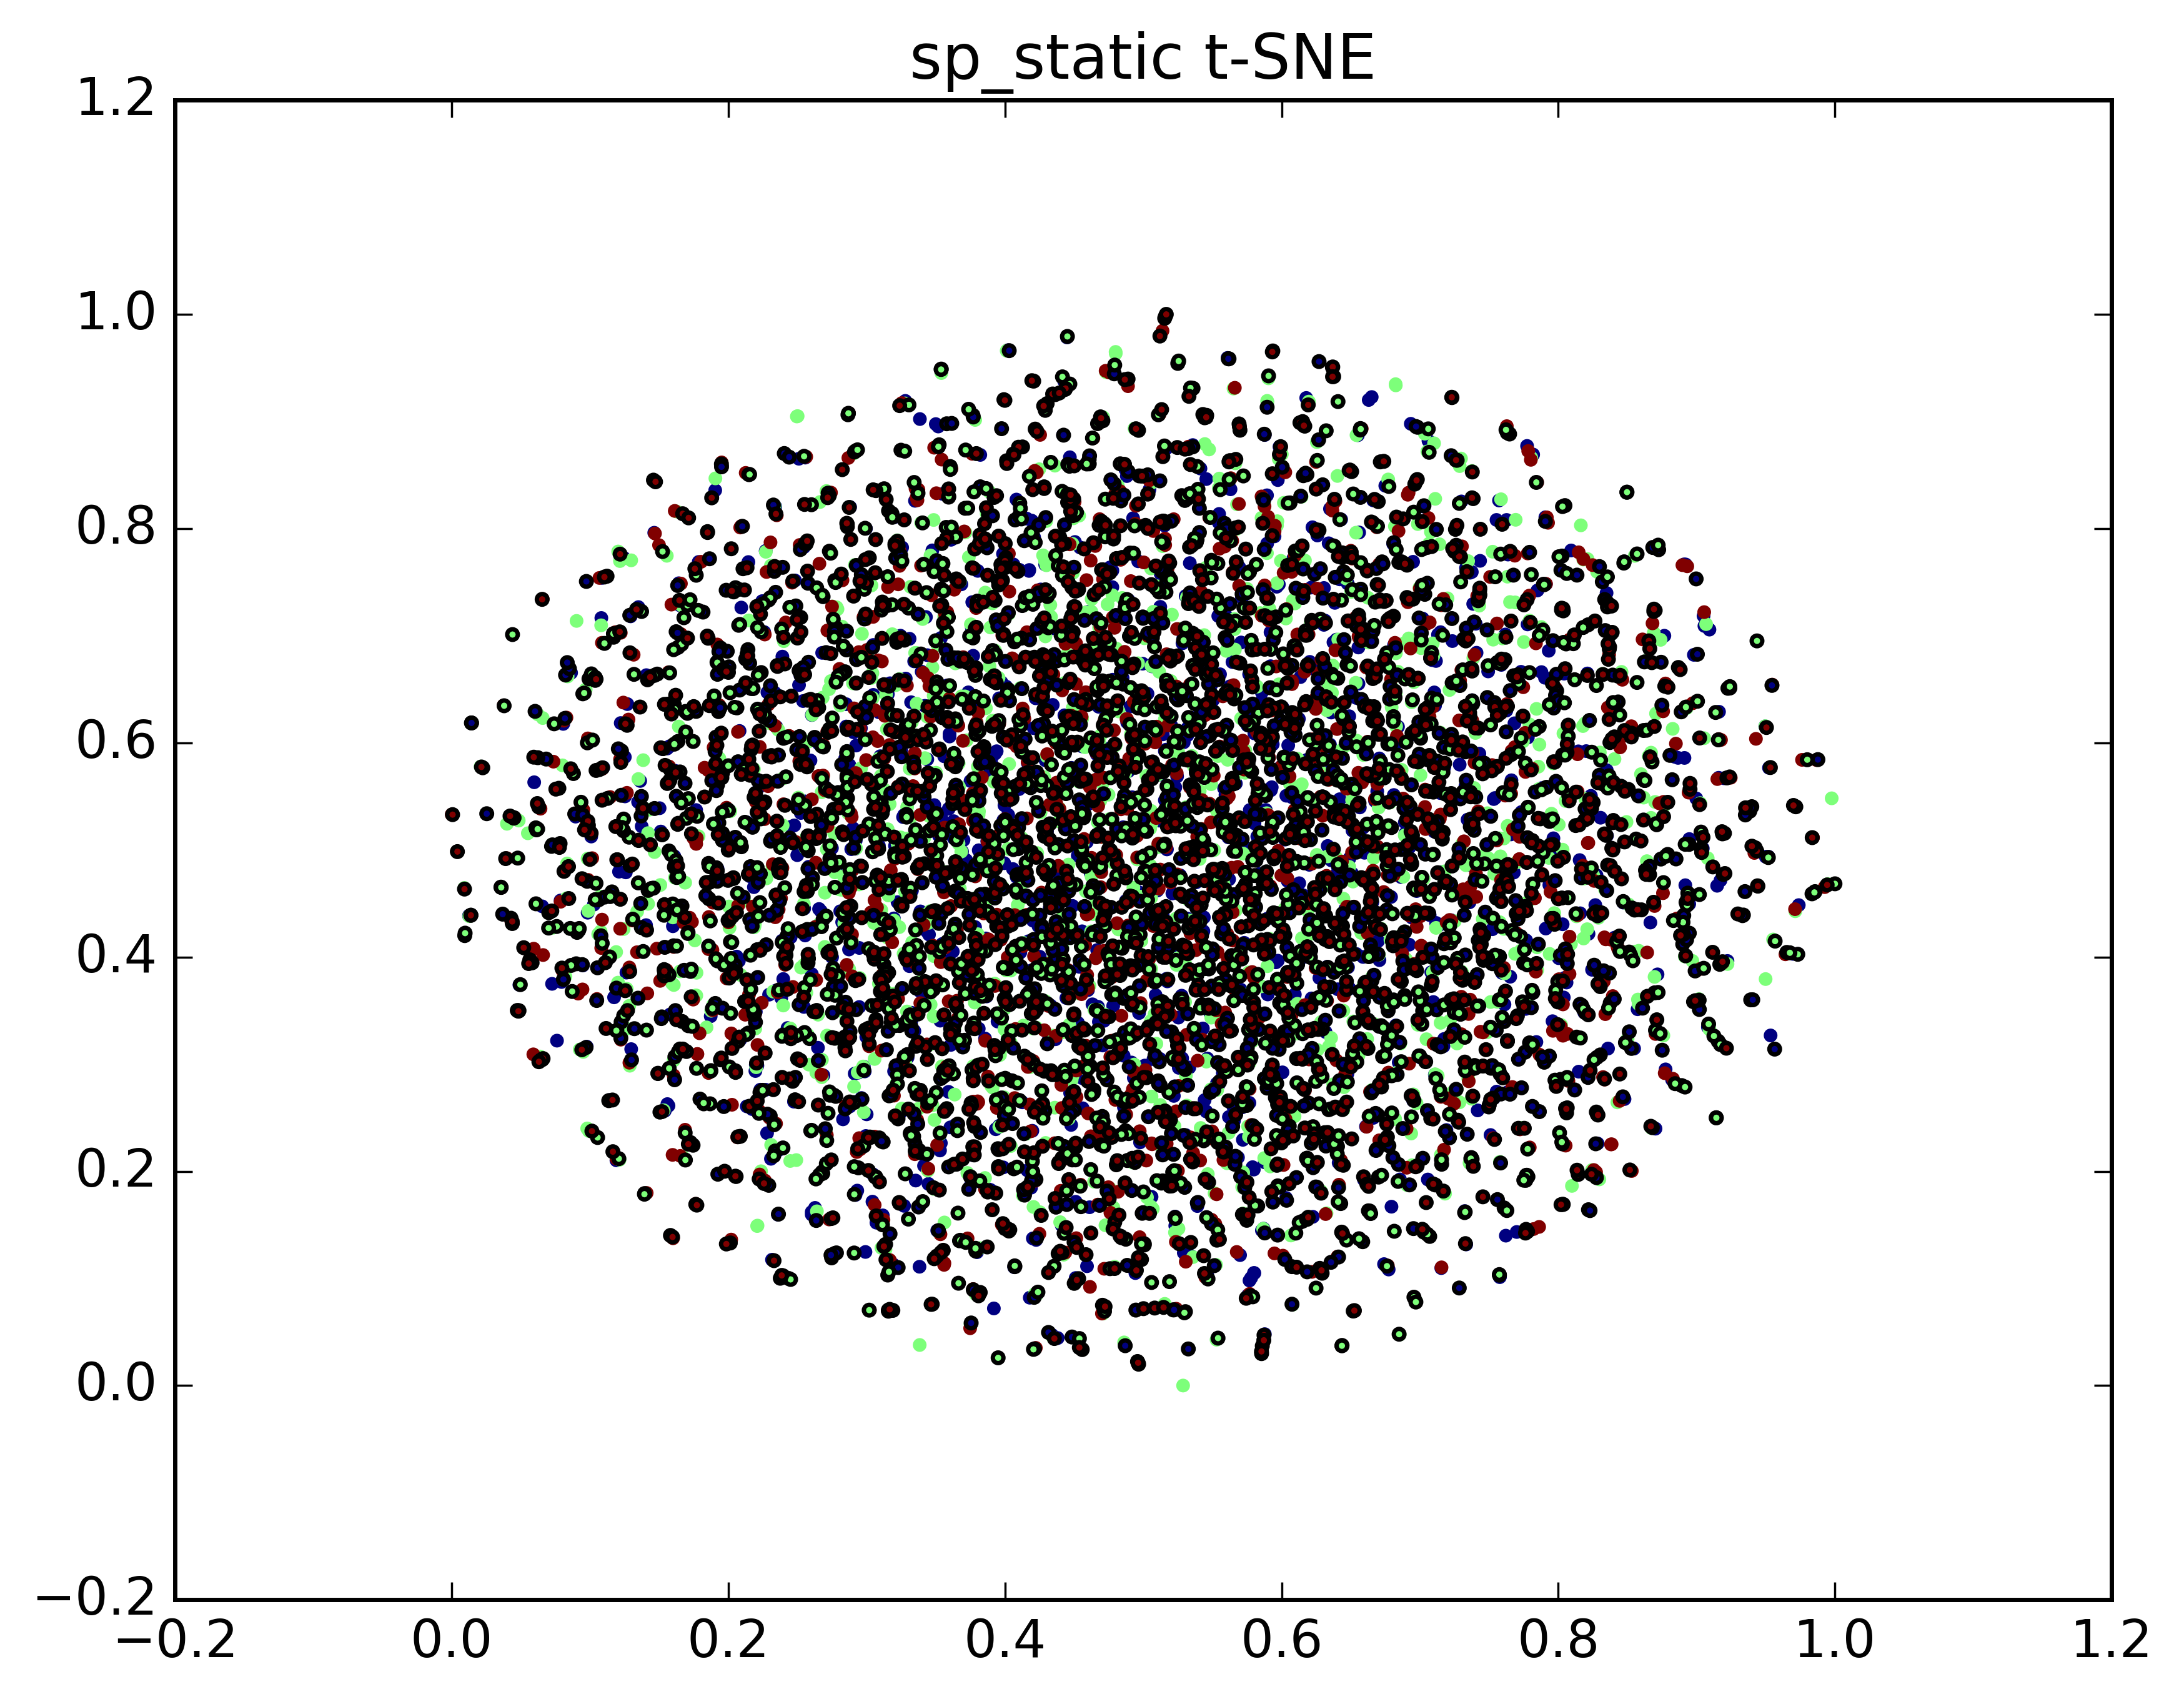
\includegraphics[width=0.8\textwidth, trim={2cm 2cm 2cm 2.5cm},clip]{images/nocluster.png}
		\end{figure}
	\end{columns}
	
\end{frame}

\begin{frame}
	\frametitle{Analyzing the data using t-SNE}
	\textbf{Visualizing EMG data using t-SNE}
	\begin{columns}
		\column{.7\textwidth}
		\begin{figure}[ht]
			\centering
			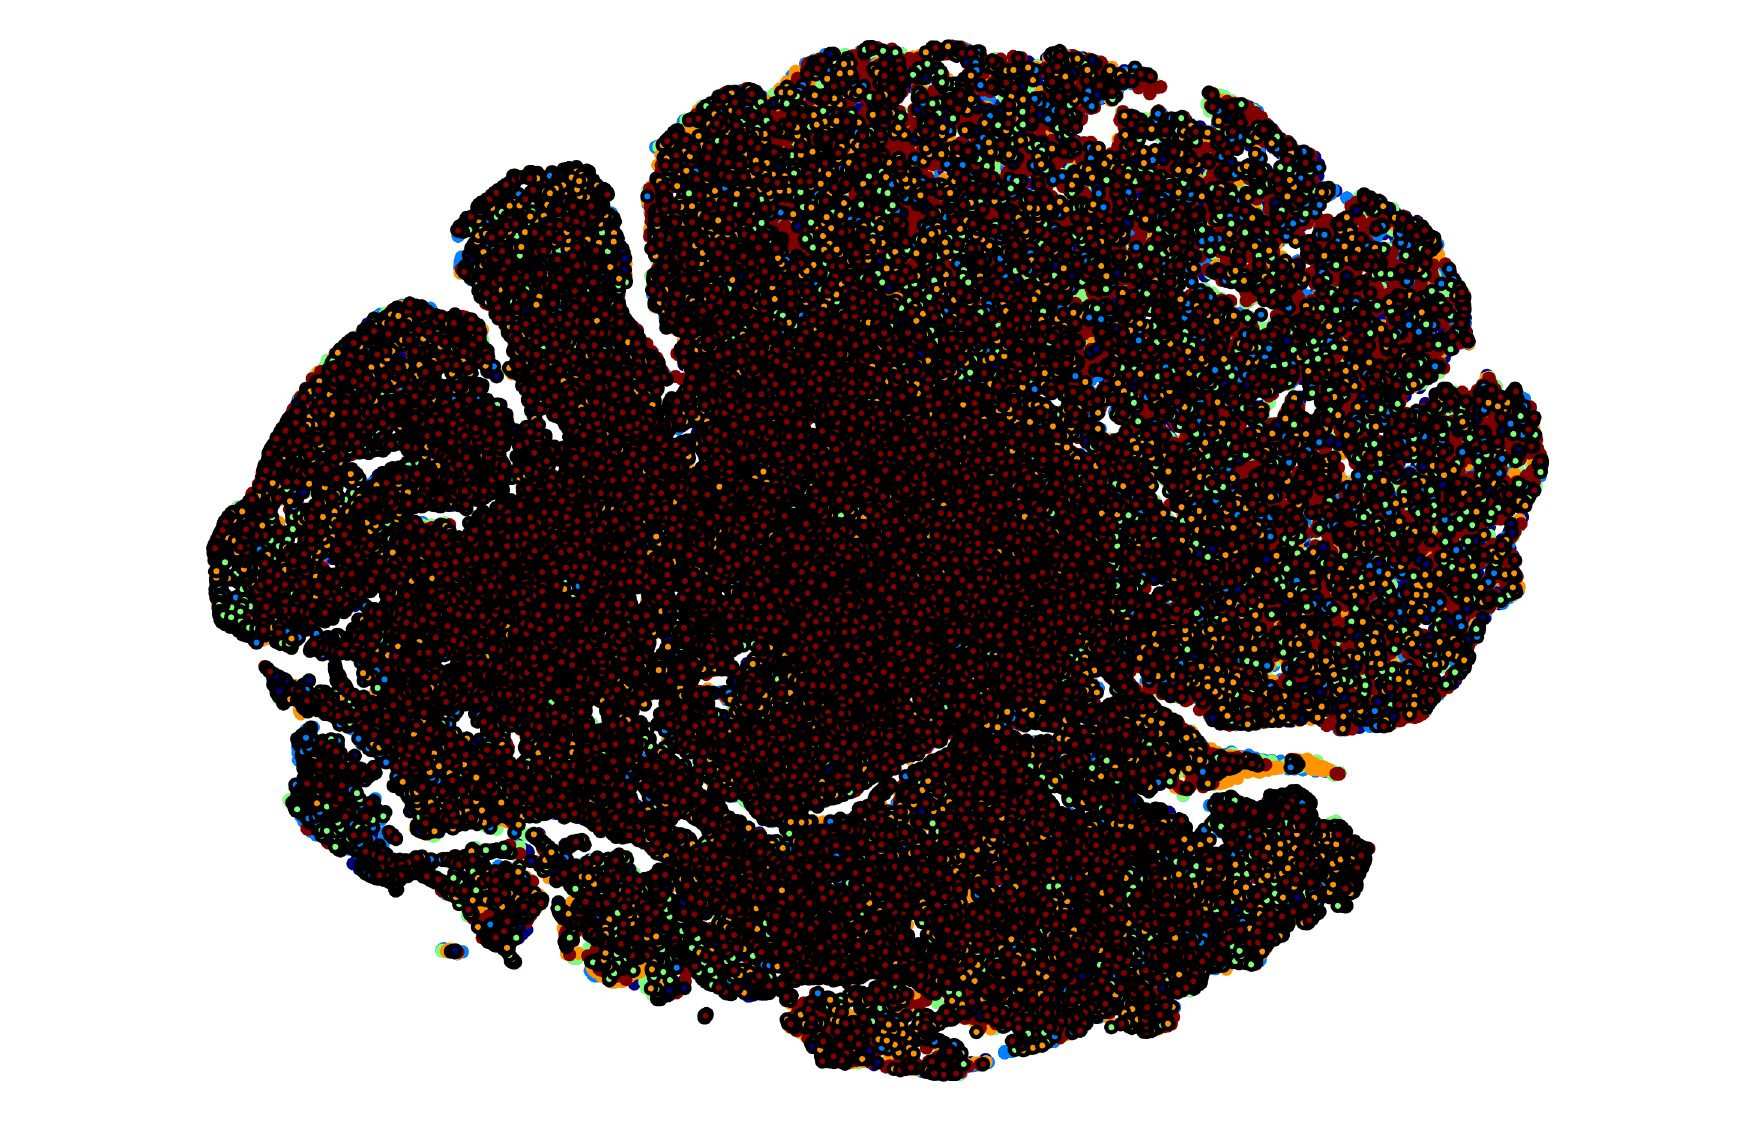
\includegraphics[width=1.0\textwidth, trim={1.5cm 0cm 1.5cm 0cm},clip]{images/emg_tsne.png}
		\end{figure}
		
		\column{.3\textwidth}
		\textbf{Attributes}
		\begin{itemize}
			\item Data of 34 trials
			\item Each colour stands for one trial
			\item Black spots mark \emph{Grasping}-states
		\end{itemize}
		\begin{block}{Conclusion}
			No apparent structure $\rightarrow$ Feedforward NN not sufficient, use Recurrent NN instead.
		\end{block}		
	\end{columns}	
\end{frame}

\begin{frame}
	\frametitle{Analysing the data using t-SNE}
	\textbf{Visualizing EEG data using t-SNE}
	\begin{columns}
		\column{.7\textwidth}
		\begin{figure}[ht]
			\centering
			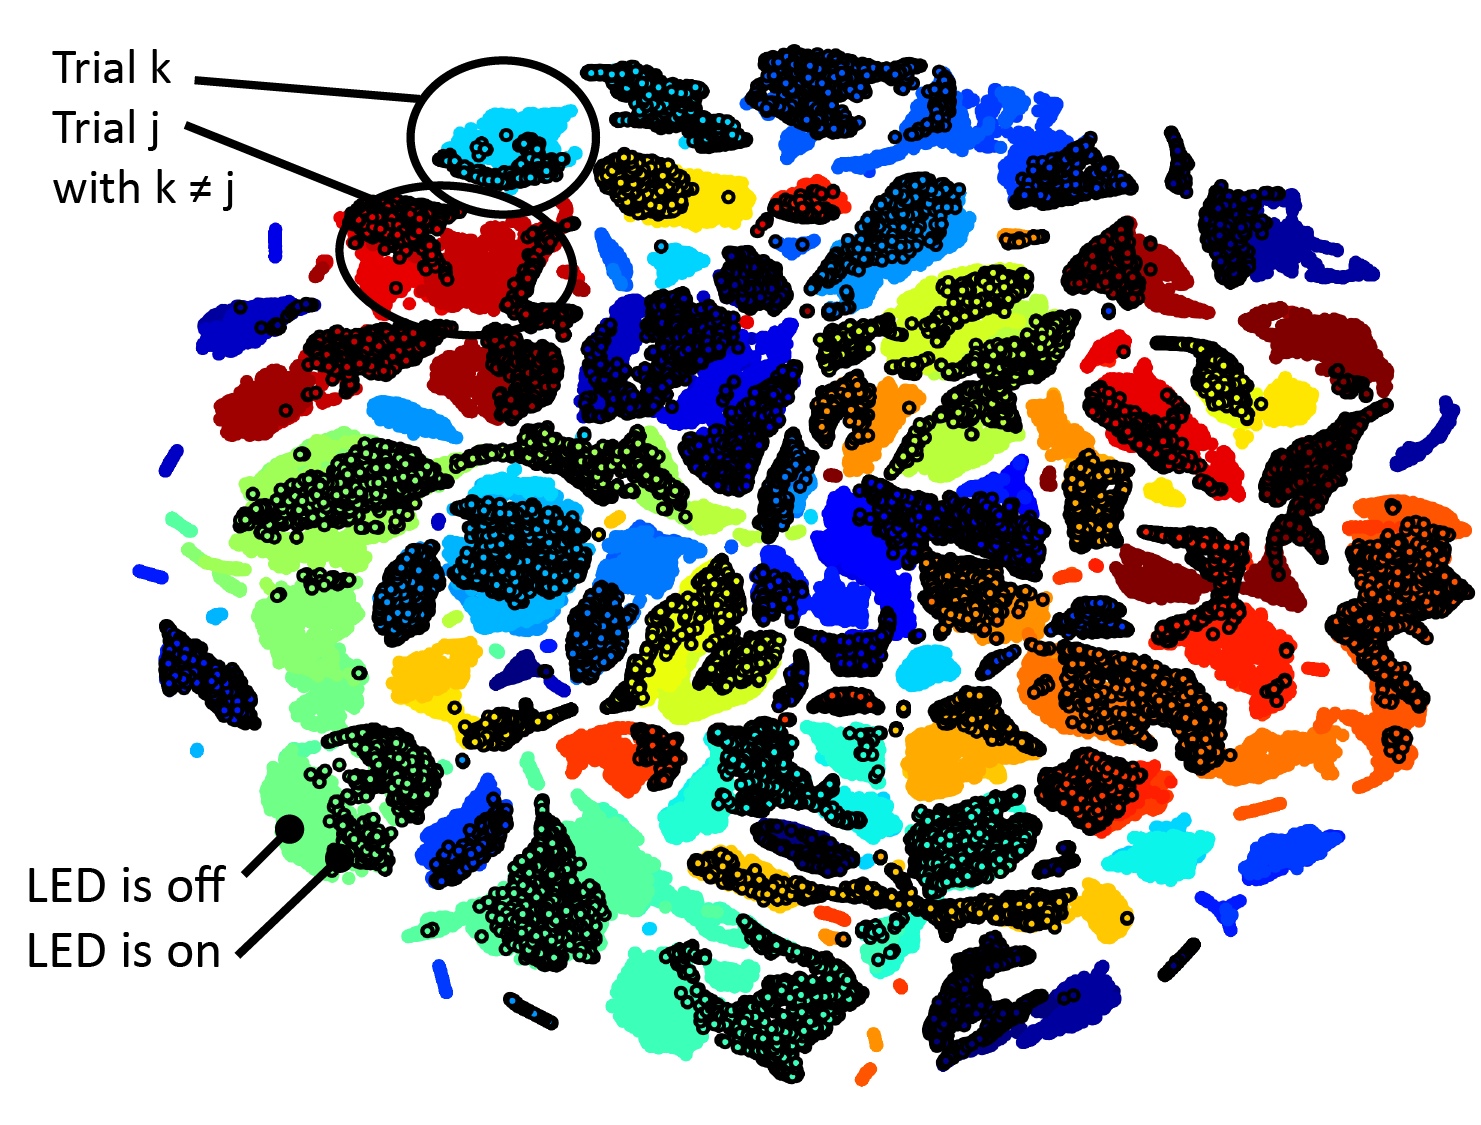
\includegraphics[width=1.0\textwidth, trim={0cm 0cm 0cm 0cm},clip]{images/eeg_tsne.png}
		\end{figure}
		
		\column{.3\textwidth}
		\textbf{Attributes}
		\begin{itemize}
			\item Data of 34 trials
			\item Each colour stands for one trial
			\item Black spots mark \emph{Grasping}-states
		\end{itemize}
		\begin{block}{Conclusion}
			Trials cluster $\rightarrow$ Weird? Use Feedforward NN to classify trials?
		\end{block}		
	\end{columns}
\end{frame}

%\begin{frame}
	%\frametitle{Classifying trials using a NN}
	%\textbf{Further analysis of EEG data}
	%\begin{block}{Verifying correct function of implementation}
		%Check code over and over, use reference data sets to make sure the plot is indeed correct $\rightarrow$ Everything seems fine
	%\end{block}
	
	%\begin{columns}
		%\column{.6\textwidth}
		%\textbf{If there is some truth to the t-SNE plot, classification of trials should be possible}
		%\begin{block}{Classify trials using a Feedforward NN}
			%Feedforward NN with:
			%\begin{itemize}
				%\item 32 EEG electrodes as input
				%\item 300 tanh-activated hidden neurons
				%\item 34 trials as output classes
			%\end{itemize}
		%\end{block}
		
		%\column{.4\textwidth}
		%\begin{figure}[ht]
			%\centering
			%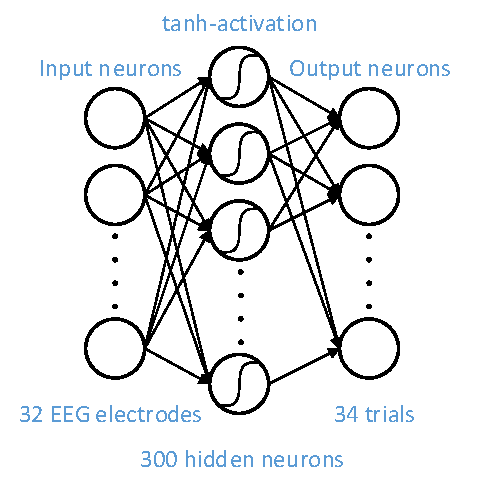
\includegraphics[width=1.0\textwidth, trim={0cm 0cm 0cm 0cm},clip]{images/FNN.pdf}
		%\end{figure}	
	%\end{columns}
%\end{frame}

\begin{frame}
	\frametitle{Results of the data analysis}
	
	\begin{block}{Results of trial classification}
		Depending on participant and series nearly perfect classification with up to just about 0.01\% error on test set.\\
		Even when classifying all participant 1's 296 trials still a good test error of about 15\% was achieved.
	\end{block}
	
	\begin{block}{Conclusion}
		We conclude that there indeed has to be some kind structure encoding the time of measurement within the EEG data.
		Also, this structure is not bound by single series but seems to be of global nature.
	\end{block}
	
	\begin{block}{Furthermore...}
		Also somewhat possible to classify the \emph{intention to grasp} (LED on states). Using the NN a test error of about 9\% was achieved.
	\end{block}
\end{frame}



%------------------------------------------------
\section{Methodology}

\begin{frame}{Methodology RNN}
        \only<1>{
                \begin{block}{Why RNNs?}
                    Assuming predictability in human action $\rightarrow$ history matters
                \end{block}

                \vspace{10px}
                \textbf{Development environment}
                \begin{itemize}
                    \item Python, Theano, Climin, Breze, Matlab, C
                \end{itemize}

                \vspace{10px}
                \textbf{Data preprocessing}
                \begin{itemize}
                    \item Input normalization to [-1;1] range
                    \item Separation into subsets of 300 timesteps length
                        \item EMG data subsampling at 10Hz
                        \item Cross validation split: train/validation/test $\rightarrow$ 0.8/0.1/0.1
                \end{itemize}
        }
        \only<2-3>{
                \begin{columns}
                        \begin{column}{0.5\textwidth}
                        \textbf{Recurrent Neural Network}
                                \begin{itemize}
                                        \item deep network with recurrent connected neurons
                                        \item suitable for sequential data
                                        \item vanishing gradient exponentially worse
                                        \item decay information over time
                                \end{itemize}
                        \end{column}
                        \begin{column}{0.5\textwidth}
                                \only<2>{
                                        \begin{figure}
                                                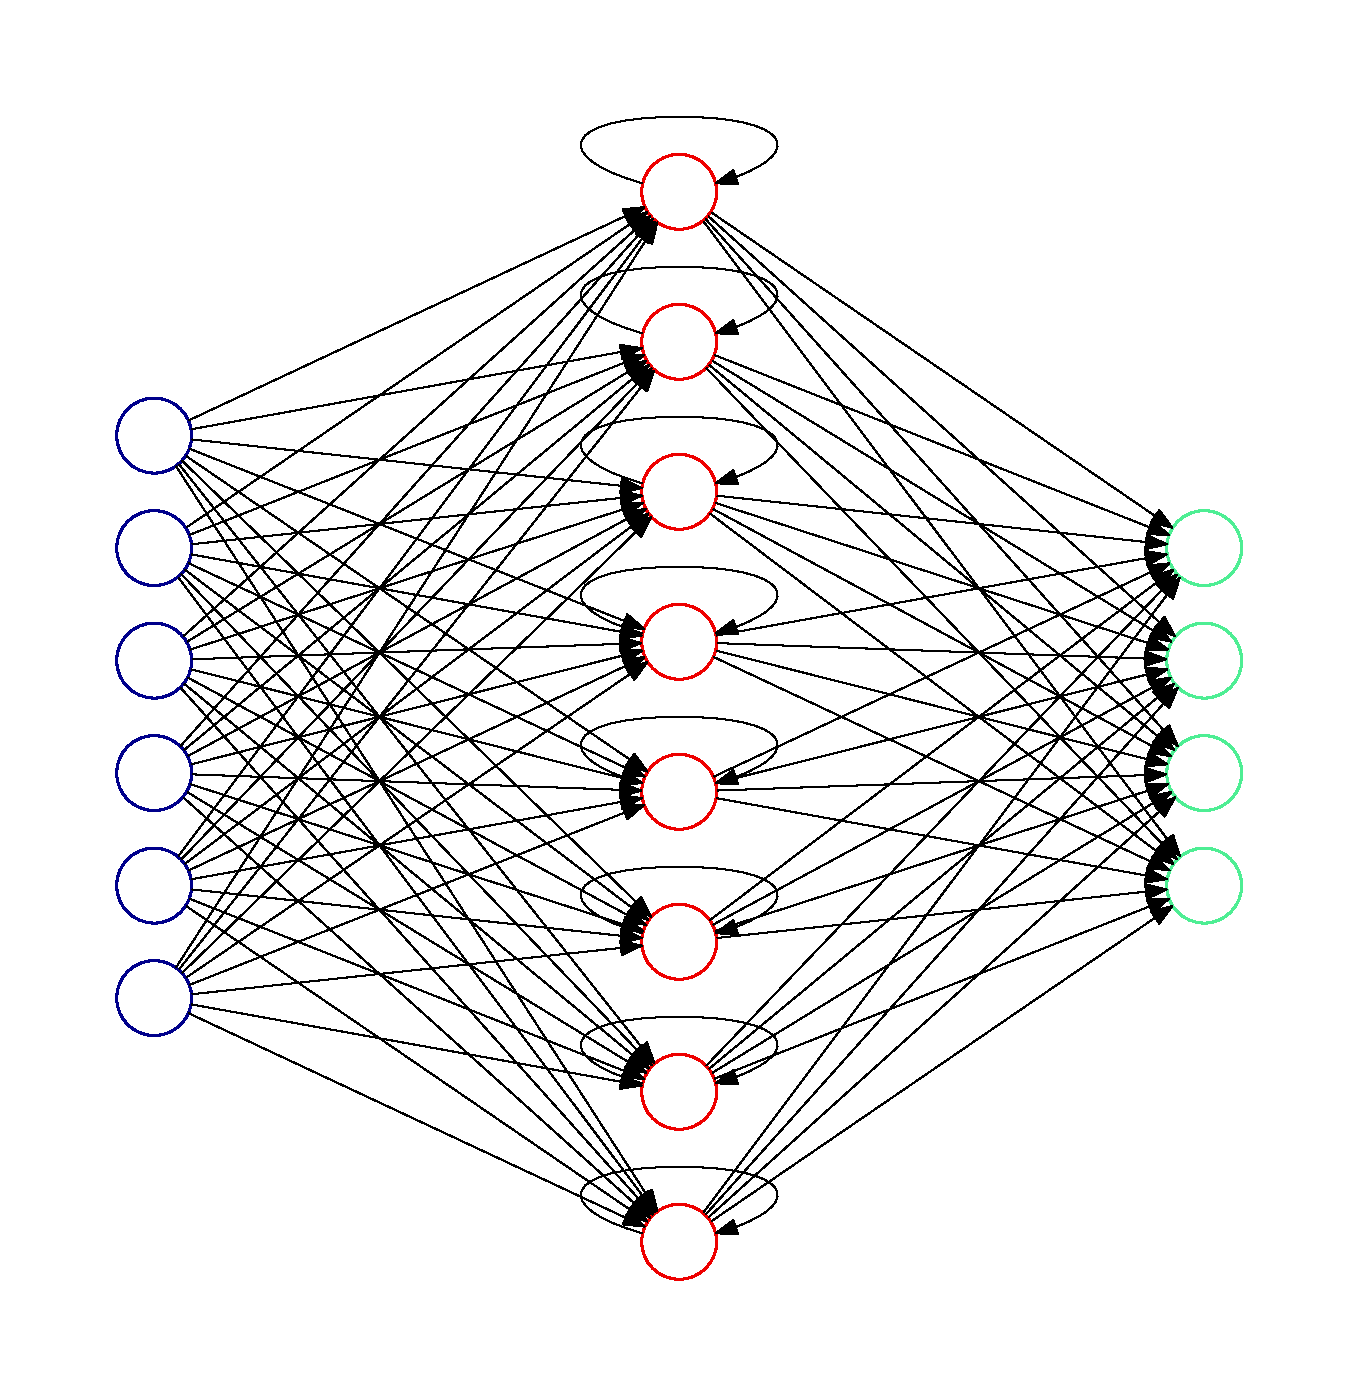
\includegraphics[width=.8\linewidth]{images/rnn_net.pdf}
                                        \end{figure}
                                }
                                \only<3>{
                                        \begin{figure}
                                                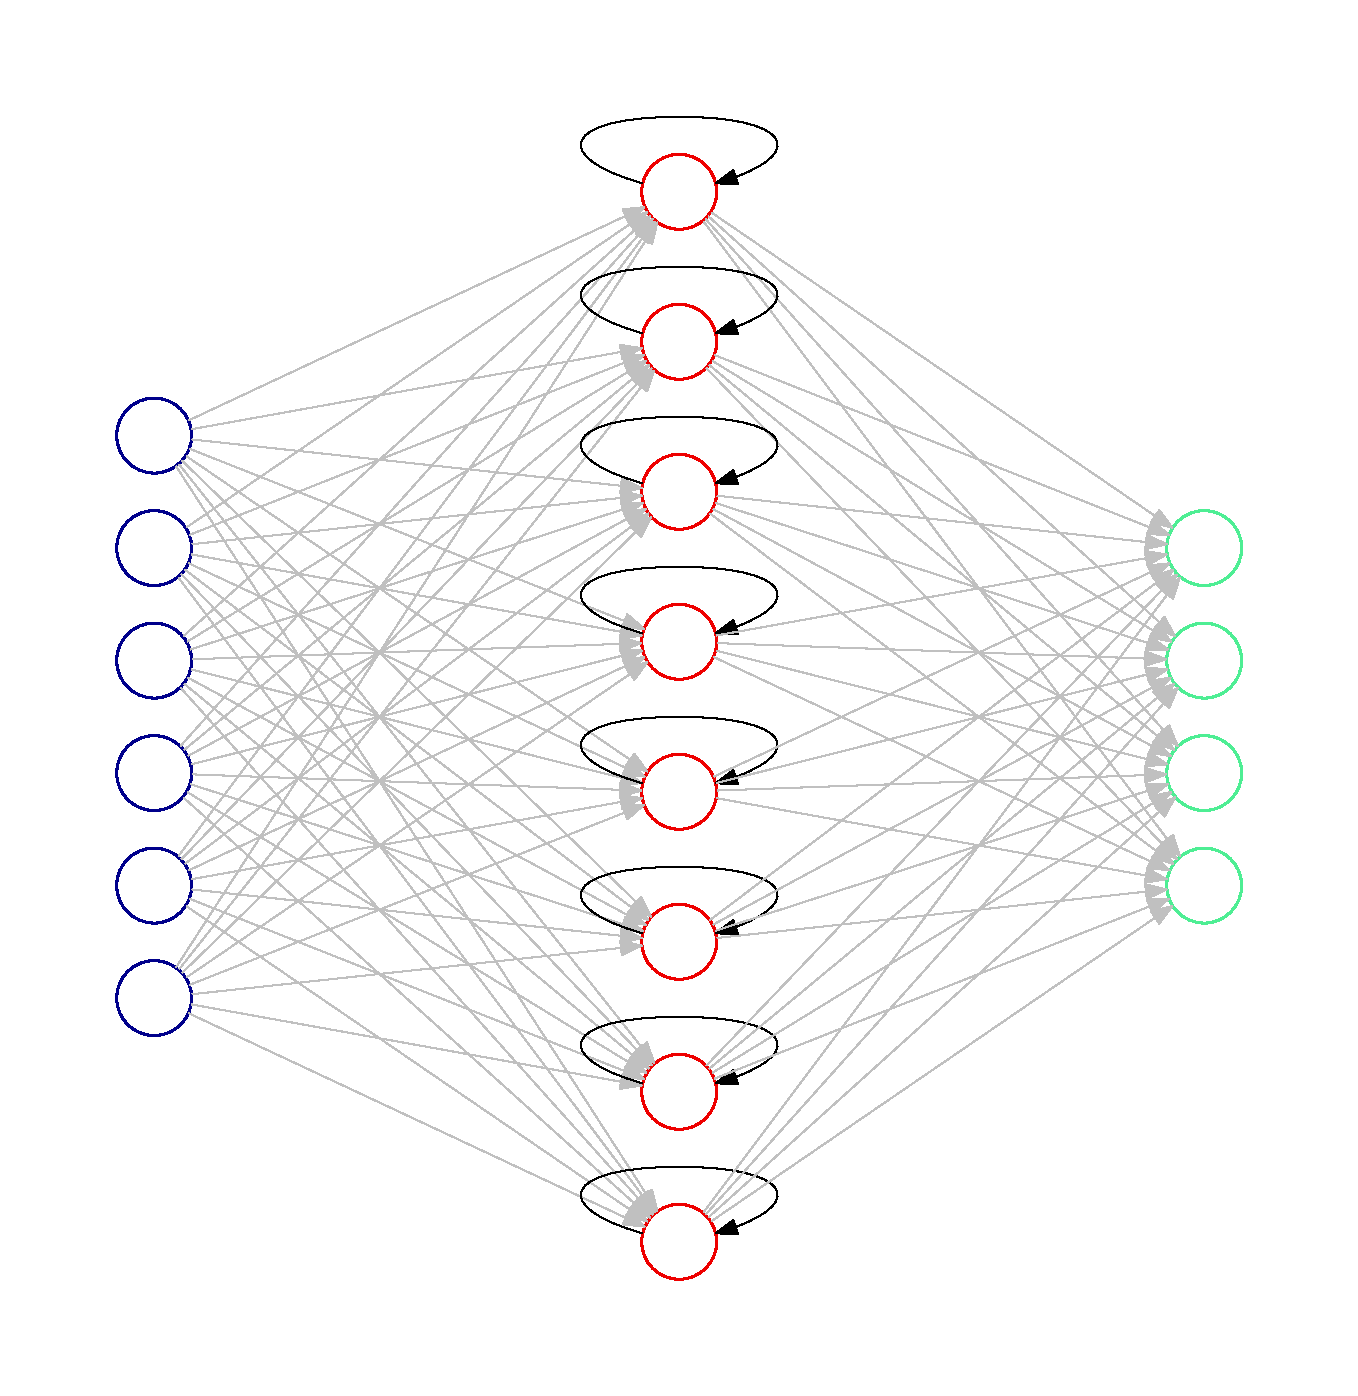
\includegraphics[width=.8\linewidth]{images/rnn_net_hl.pdf}
                                        \end{figure}
                                }
                        \end{column}
                \end{columns}
        }
        \only<4>{
                \textbf{Recurrent Neural Network}
                \begin{itemize}
                    \item Network design:
                    \begin{itemize}
                        \item 100/200 tanh activated neurons in 1 hidden layer
                        \item sigmoidal output neurons
                        \item 50 samples per batch
                        \item optimizer: Adadelta, \(RmsProp\)
                    \end{itemize}
                    \item Weights initialization by random uniform distribution
                %    \item spectral radius
                    \item Important weights: 150
                %    \begin{itemize}
                %        \item some samples are more important to learn than others
                %        \item skip first ~150 samples till transient oscillation
                %    \end{itemize}
                    \item Bernoulli cross entropy loss
                \end{itemize}
        }
        \only<5>{
                \textbf{Targets}
                \begin{columns}
                	\begin{column}{0.5\textwidth}
                \begin{itemize}
                        \item one-hot-encoding
                    \item defined by given events:
                    \begin{enumerate}
                    \item Move hand to target phase
                    \item lift object phase
                    \item hold object phase
                    \item replace object phase
                    \item Move hand back to start phase
                        %\item move hand to start
                %        \item touch object phase
                    \end{enumerate}
                \end{itemize}
                \end{column}
                \begin{column}{0.5\textwidth}

                    \begin{figure}[ht]
                    	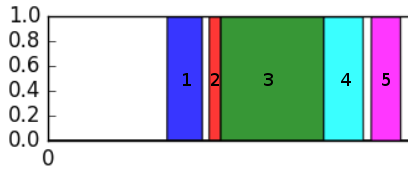
\includegraphics[width=1.0\linewidth]{images/targets.png}
                    \end{figure}
                \end{column}
            \end{columns}

                %    \item Data shape
                %    \begin{itemize}
                %        \item Input: [time slice, features, sensors] $\rightarrow$ [300 x 2428 x 5/32]
                %        \item Target: [time slice, features, targets] $\rightarrow$ [300 x 1320 x 1]
                %%        \item format given as breze requirement \textbf{(Does anyone in the audience care?)}
                %    \end{itemize}


                %LSTM
                %\begin{itemize}
                %    \item usage of breze library implementation \footnote{https://github.com/breze-no-salt/breze v0.1 (2016)} 
                %    \item finally not used because satisfying results achivable by RNN
                %\end{itemize}
        }
\end{frame}


\section{RNN results}		

\begin{frame}
	\frametitle{Results of RNN: EMG data}
	\textbf{Training with data of one participant}
	\begin{figure}[ht]
		\centering
		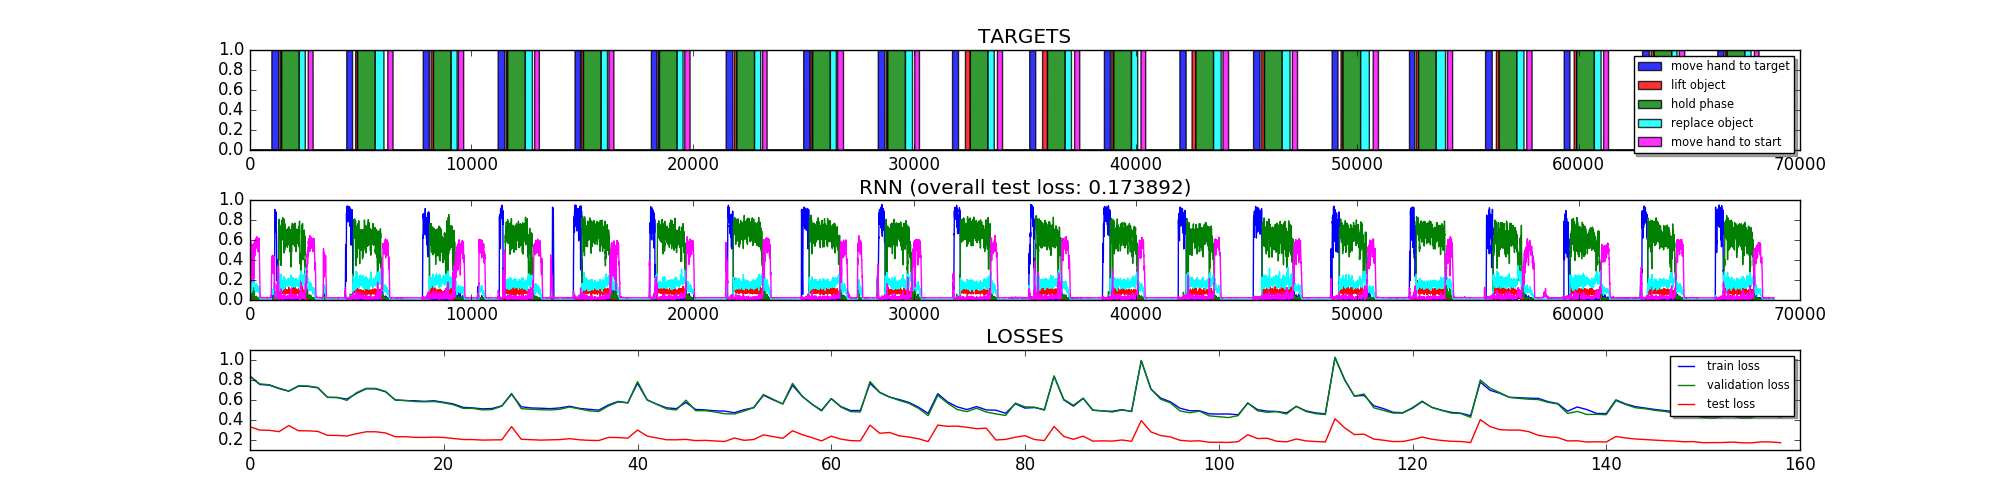
\includegraphics[width=1.0\textwidth,trim={5cm 0cm 5cm 0cm},clip]{images/EMG-results_participant_1_series1-6.png}
		\caption{Results of RNN trained with data of participant 1, series 1-6}
	\end{figure}
\end{frame}

\begin{frame}
	\frametitle{Results of RNN: EMG data}
	\textbf{Training with data of more than one participant}
	\begin{figure}[ht]
		\centering
		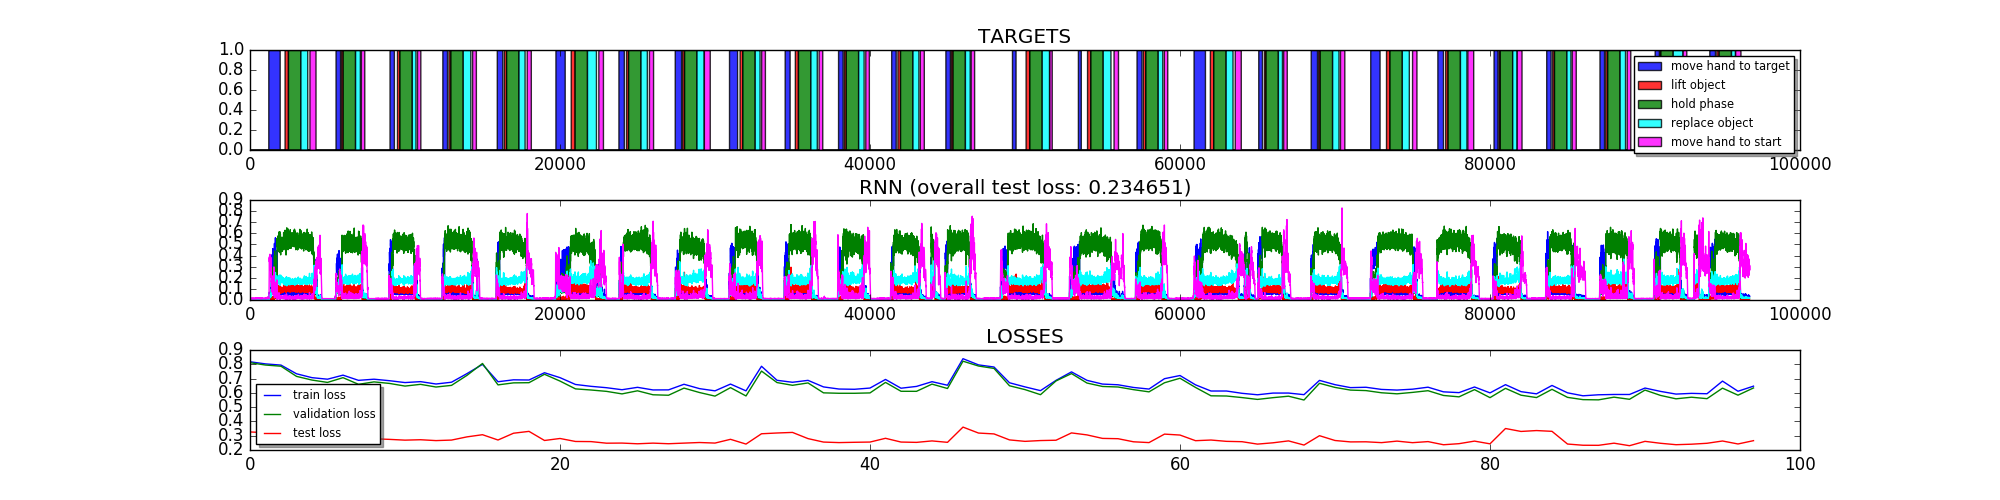
\includegraphics[width=1.0\textwidth,trim={5cm 0cm 5cm 0cm},clip]{images/EMG-results_participant_1-4_series1-2.png}
		\caption{Results of RNN trained with data of participants 1-4, series 1-2}

	\end{figure}
\end{frame}

\begin{frame}
	\frametitle{Results of RNN: EEG data}
	\textbf{Training with data of one participant - one target}
	\begin{figure}[ht]
		\centering
		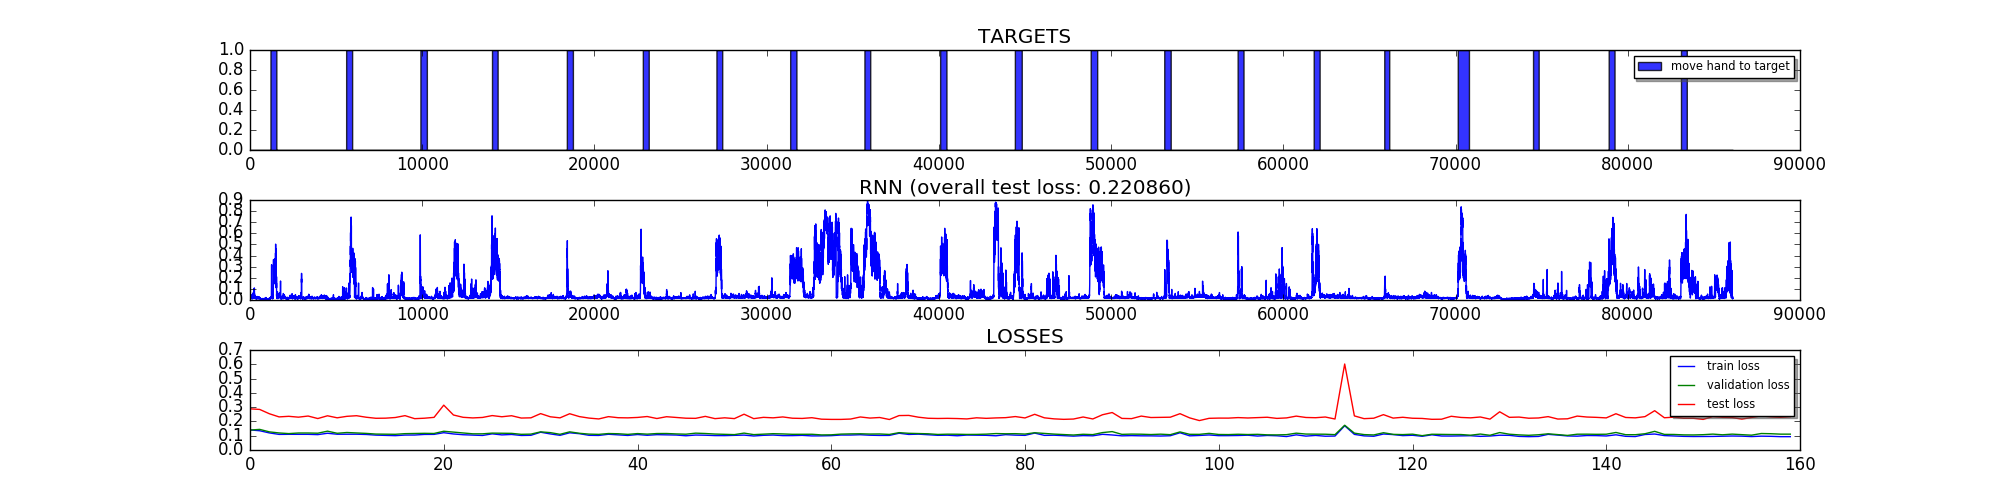
\includegraphics[width=1.0\textwidth,trim={5cm 0cm 5cm 0cm},clip]{images/200_50_[1]_[1,2,3,4,5,6]_0_150_1_1469550907_eeg_test.png}
		\caption{Results of RNN trained with data of participant 1, series 1-6}

	\end{figure}
\end{frame}

\begin{frame}
	\frametitle{Results of RNN: EEG data}
	\textbf{Training with data of more than one participant - one target}
	\begin{figure}[ht]
		\centering
		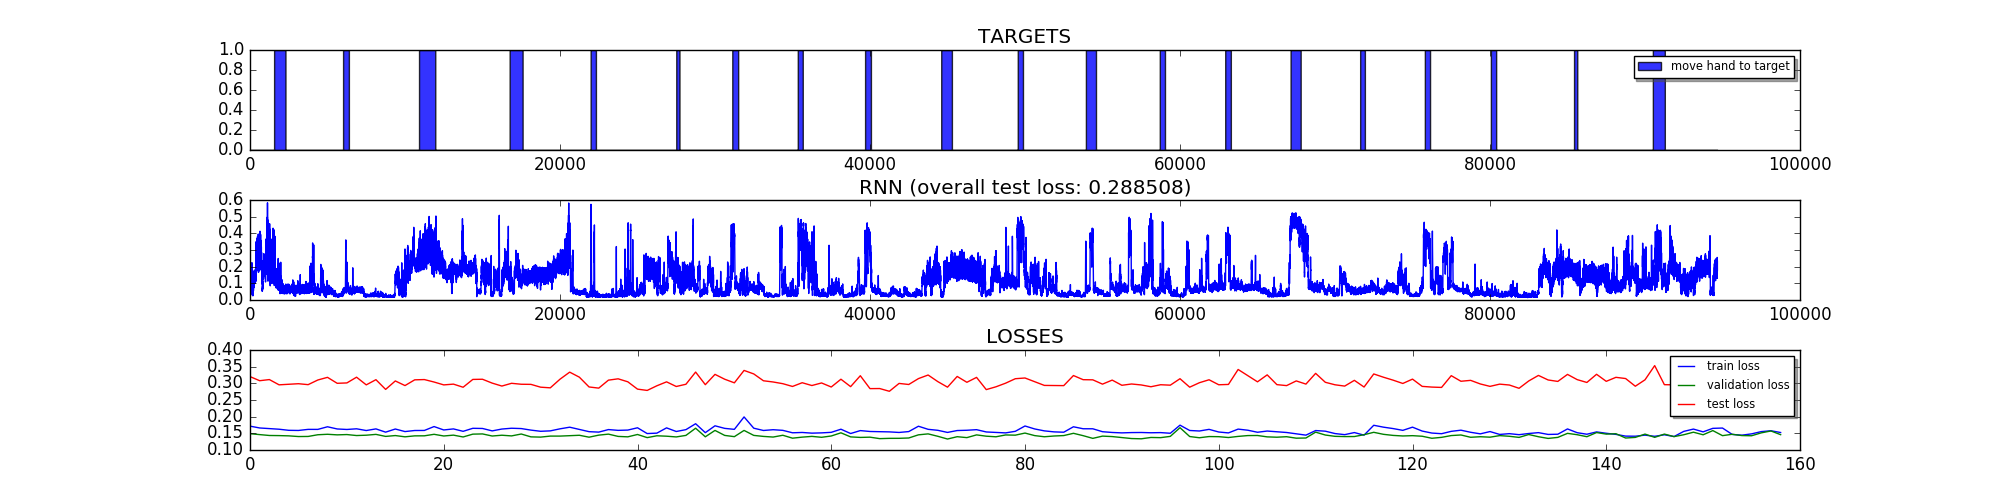
\includegraphics[width=1.0\textwidth,trim={5cm 0cm 5cm 0cm},clip]{images/200_50_[1,2]_[1,2,3]_0_150_1_1469542956_eeg_test.png}
		\caption{Results of RNN trained with data of participants 1-2, series 1-3}

	\end{figure}
\end{frame}

\begin{frame}
	\frametitle{Results of RNN: EEG data}
	\textbf{Training with data of one participant - multiple targets}
	\begin{figure}[ht]
		\centering
		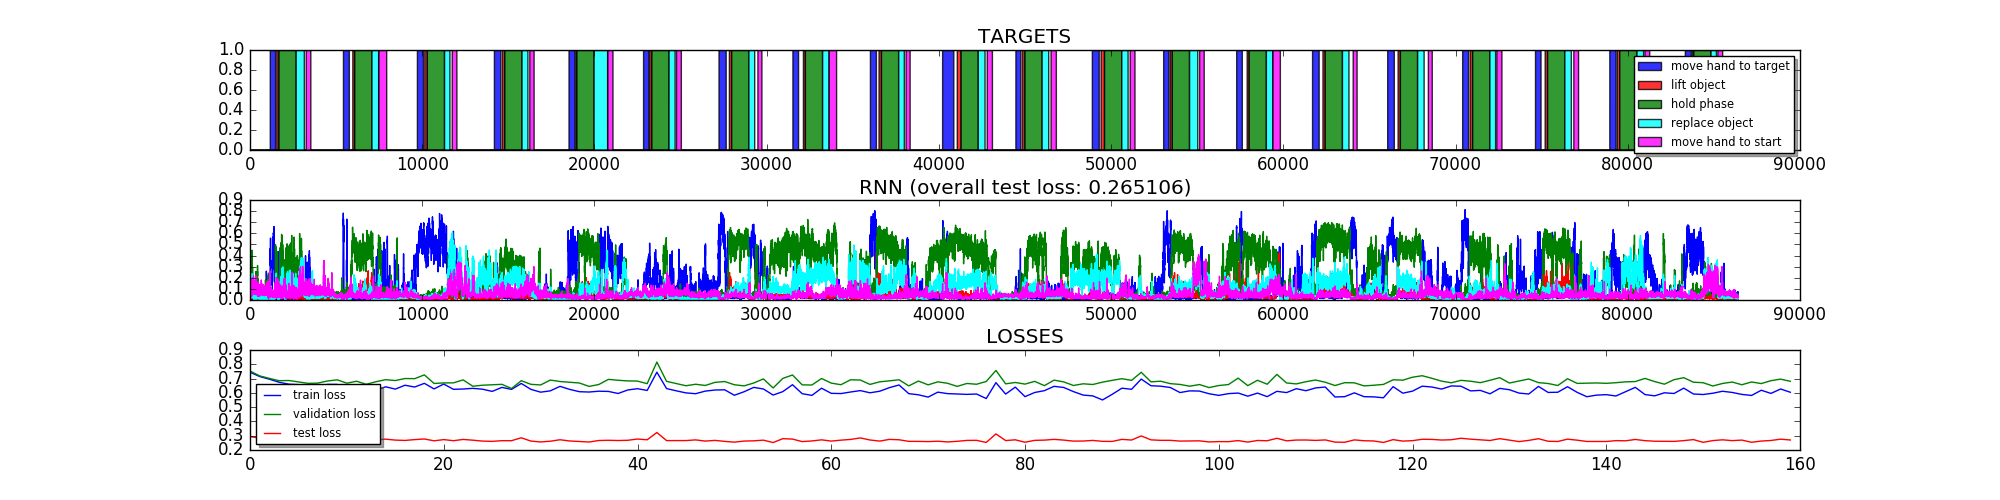
\includegraphics[width=1.0\textwidth,trim={5cm 0cm 5cm 0cm},clip]{images/200_50_[1]_[1,2,3,4,5,6]_0_150_1_1469560909_eeg_test.png}
		\caption{Results of RNN trained with data of participant 1, series 1-6}

	\end{figure}
\end{frame}

%------------------------------------------------
\section{Pitfalls}

\begin{frame}
	\frametitle{Pitfalls}
	\begin{itemize}
		%\item No working early stopping criterion (so far)
		\item Huge amount of data
		\item Limitations through Hardware
		\item Different recording frequencies
		\item Timespans of Targets "lift object" and "replace object" very short
        %\item Equalization of different length records
        %\begin{itemize}
        %    \item zero padding $\rightarrow$ learning in danger of being misguided
        %    \item tail cut $\rightarrow$ targets fall of, fails to learn sometimes
        %\end{itemize}
        \item Predictions do not fit to the target borders exactly
        \item Test loss by constant factor smaller/bigger than train and validation loss
	\end{itemize}
\end{frame}

%------------------------------------------------

\begin{frame}
%\frametitle{The End}
\begin{center}
	\textbf{\Huge{Thank You!}}
\end{center}
\end{frame}

%%------------------------------------------------

%\begin{frame}
%\frametitle{Blocks of Highlighted Text}
%\begin{block}{Block 1}
%Lorem ipsum dolor sit amet, consectetur adipiscing elit. Integer lectus nisl, ultricies in feugiat rutrum, porttitor sit amet augue. Aliquam ut tortor mauris. Sed volutpat ante purus, quis accumsan dolor.
%\end{block}

%\begin{block}{Block 2}
%Pellentesque sed tellus purus. Class aptent taciti sociosqu ad litora torquent per conubia nostra, per inceptos himenaeos. Vestibulum quis magna at risus dictum tempor eu vitae velit.
%\end{block}

%\begin{block}{Block 3}
%Suspendisse tincidunt sagittis gravida. Curabitur condimentum, enim sed venenatis rutrum, ipsum neque consectetur orci, sed blandit justo nisi ac lacus.
%\end{block}
%\end{frame}

%%------------------------------------------------

%\begin{frame}
%\frametitle{Multiple Columns}
%\begin{columns}[c] % The "c" option specifies centered vertical alignment while the "t" option is used for top vertical alignment

%\column{.45\textwidth} % Left column and width
%\textbf{Heading}
%\begin{enumerate}
%\item Statement
%\item Explanation
%\item Example
%\end{enumerate}

%\column{.5\textwidth} % Right column and width
%Lorem ipsum dolor sit amet, consectetur adipiscing elit. Integer lectus nisl, ultricies in feugiat rutrum, porttitor sit amet augue. Aliquam ut tortor mauris. Sed volutpat ante purus, quis accumsan dolor.

%\end{columns}
%\end{frame}

%\begin{frame}
%\frametitle{Table}
%\begin{table}
%\begin{tabular}{l l l}
%\toprule
%\textbf{Treatments} & \textbf{Response 1} & \textbf{Response 2}\\
%\midrule
%Treatment 1 & 0.0003262 & 0.562 \\
%Treatment 2 & 0.0015681 & 0.910 \\
%Treatment 3 & 0.0009271 & 0.296 \\
%\bottomrule
%\end{tabular}
%\caption{Table caption}
%\end{table}
%\end{frame}

%%------------------------------------------------

%\begin{frame}
%\frametitle{Theorem}
%\begin{theorem}[Mass--energy equivalence]
%$E = mc^2$
%\end{theorem}
%\end{frame}

%%------------------------------------------------

%\begin{frame}[fragile] % Need to use the fragile option when verbatim is used in the slide
%\frametitle{Verbatim}
%\begin{example}[Theorem Slide Code]
%\begin{verbatim}
%\begin{frame}
%\frametitle{Theorem}
%\begin{theorem}[Mass--energy equivalence]
%$E = mc^2$
%\end{theorem}
%\end{frame}\end{verbatim}
%\end{example}
%\end{frame}

%%------------------------------------------------

%\begin{frame}
%\frametitle{Figure}
%Uncomment the code on this slide to include your own image from the same directory as the template .TeX file.
%%\begin{figure}
%%\includegraphics[width=0.8\linewidth]{test}
%%\end{figure}
%\end{frame}

%%------------------------------------------------

%\begin{frame}[fragile] % Need to use the fragile option when verbatim is used in the slide
%\frametitle{Citation}
%An example of the \verb|\cite| command to cite within the presentation:\\~

%This statement requires citation \cite{p1}.
%\end{frame}

%%------------------------------------------------

\begin{frame}
\frametitle{References}
\footnotesize{
    \begin{thebibliography}{99} % Beamer does not support BibTeX so references must be inserted manually as below
%        \bibitem[Smith, 2012]{p1} John Smith (2012)
%        \newblock Title of the publication
%        \newblock \emph{Journal Name} 12(3), 45 -- 678.

        \bibitem[nature]{nature} Matthew D Luciw, Ewa Jarocka \& Benoni B Edin
        \newblock Multi-channel EEG recordings during 3,936 grasp and lift trials with varying weight and friction
        \newblock \emph http://www.nature.com/articles/sdata201447, requested at: July 26th 2016
      
        \bibitem[EEG-GAL, 2014]{eeg-emg-dataset} Luciw, M. D., Jarocka, E. \& Edin, B. B.  (2014)
        \newblock Data set: WAY-EEG-GAL 
        \newblock \emph FigShare http://dx.doi.org/10.6084/m9.figshare.988376, requested at: July 26th 2016
        
    \end{thebibliography}
}
\end{frame}

%%------------------------------------------------
%
%\begin{frame}
%\Huge{\centerline{The End}}
%\end{frame}

%----------------------------------------------------------------------------------------

\end{document} 
